\documentclass[9pt,a4paper,]{extarticle}

\usepackage{f1000_styles}

\usepackage[pdfborder={0 0 0}]{hyperref}

\usepackage[numbers]{natbib}
\bibliographystyle{unsrtnat}


%% maxwidth is the original width if it is less than linewidth
%% otherwise use linewidth (to make sure the graphics do not exceed the margin)
\makeatletter
\def\maxwidth{ %
  \ifdim\Gin@nat@width>\linewidth
    \linewidth
  \else
    \Gin@nat@width
  \fi
}
\makeatother

\usepackage{color}
\usepackage{fancyvrb}
\newcommand{\VerbBar}{|}
\newcommand{\VERB}{\Verb[commandchars=\\\{\}]}
\DefineVerbatimEnvironment{Highlighting}{Verbatim}{commandchars=\\\{\}}
% Add ',fontsize=\small' for more characters per line
\usepackage{framed}
\definecolor{shadecolor}{RGB}{248,248,248}
\newenvironment{Shaded}{\begin{snugshade}}{\end{snugshade}}
\newcommand{\KeywordTok}[1]{\textcolor[rgb]{0.13,0.29,0.53}{\textbf{#1}}}
\newcommand{\DataTypeTok}[1]{\textcolor[rgb]{0.13,0.29,0.53}{#1}}
\newcommand{\DecValTok}[1]{\textcolor[rgb]{0.00,0.00,0.81}{#1}}
\newcommand{\BaseNTok}[1]{\textcolor[rgb]{0.00,0.00,0.81}{#1}}
\newcommand{\FloatTok}[1]{\textcolor[rgb]{0.00,0.00,0.81}{#1}}
\newcommand{\ConstantTok}[1]{\textcolor[rgb]{0.00,0.00,0.00}{#1}}
\newcommand{\CharTok}[1]{\textcolor[rgb]{0.31,0.60,0.02}{#1}}
\newcommand{\SpecialCharTok}[1]{\textcolor[rgb]{0.00,0.00,0.00}{#1}}
\newcommand{\StringTok}[1]{\textcolor[rgb]{0.31,0.60,0.02}{#1}}
\newcommand{\VerbatimStringTok}[1]{\textcolor[rgb]{0.31,0.60,0.02}{#1}}
\newcommand{\SpecialStringTok}[1]{\textcolor[rgb]{0.31,0.60,0.02}{#1}}
\newcommand{\ImportTok}[1]{#1}
\newcommand{\CommentTok}[1]{\textcolor[rgb]{0.56,0.35,0.01}{\textit{#1}}}
\newcommand{\DocumentationTok}[1]{\textcolor[rgb]{0.56,0.35,0.01}{\textbf{\textit{#1}}}}
\newcommand{\AnnotationTok}[1]{\textcolor[rgb]{0.56,0.35,0.01}{\textbf{\textit{#1}}}}
\newcommand{\CommentVarTok}[1]{\textcolor[rgb]{0.56,0.35,0.01}{\textbf{\textit{#1}}}}
\newcommand{\OtherTok}[1]{\textcolor[rgb]{0.56,0.35,0.01}{#1}}
\newcommand{\FunctionTok}[1]{\textcolor[rgb]{0.00,0.00,0.00}{#1}}
\newcommand{\VariableTok}[1]{\textcolor[rgb]{0.00,0.00,0.00}{#1}}
\newcommand{\ControlFlowTok}[1]{\textcolor[rgb]{0.13,0.29,0.53}{\textbf{#1}}}
\newcommand{\OperatorTok}[1]{\textcolor[rgb]{0.81,0.36,0.00}{\textbf{#1}}}
\newcommand{\BuiltInTok}[1]{#1}
\newcommand{\ExtensionTok}[1]{#1}
\newcommand{\PreprocessorTok}[1]{\textcolor[rgb]{0.56,0.35,0.01}{\textit{#1}}}
\newcommand{\AttributeTok}[1]{\textcolor[rgb]{0.77,0.63,0.00}{#1}}
\newcommand{\RegionMarkerTok}[1]{#1}
\newcommand{\InformationTok}[1]{\textcolor[rgb]{0.56,0.35,0.01}{\textbf{\textit{#1}}}}
\newcommand{\WarningTok}[1]{\textcolor[rgb]{0.56,0.35,0.01}{\textbf{\textit{#1}}}}
\newcommand{\AlertTok}[1]{\textcolor[rgb]{0.94,0.16,0.16}{#1}}
\newcommand{\ErrorTok}[1]{\textcolor[rgb]{0.64,0.00,0.00}{\textbf{#1}}}
\newcommand{\NormalTok}[1]{#1}

% disable code chunks background
%\renewenvironment{Shaded}{}{}

% disable section numbers
\setcounter{secnumdepth}{0}

\setlength{\parindent}{0pt}
\setlength{\parskip}{6pt plus 2pt minus 1pt}



\begin{document}
\pagestyle{front}

\title{Enhancing gene set enrichment using networks}

\author[1]{Michael Prummer}
\affil[1]{NEXUS Personalized Health Technologies, ETH Zurich, and Swiss Institute for Bioinformatics, Zurich, Switzerland.}

\maketitle
\thispagestyle{front}

\begin{abstract}
Differential gene expression (DGE) studies often suffer from poor interpretability of their primary results, i.e., thousands of differentially expressed genes. This has led to the introduction of gene set analysis (GSA) methods that aim at identifying interpretable global effects by grouping genes into sets of common context, such as, molecular pathways, biological function or tissue localization. In practice, GSA often results in hundreds of differentially regulated gene sets. Gene sets are often regulated in a correlative fashion because they share many of their genes or they describe related processes. Using these kind of neighborhood information to construct networks of gene sets allows to identify highly connected sub-networks as well as poorly connected islands or singletons. We show here how topological information and other network features can be used to filter and prioritize gene sets in routine DGE studies. Community detection in combination with automatic labeling and the network representation of gene set clusters further constitute an appealing and intuitive visualization of GSA results. The RICHNET workflow described here does not require human intervention and can thus be conveniently incorporated in automated analysis pipelines.
\end{abstract}

\section*{Keywords}
differential gene expression analysis, gene set analysis, enrichment analysis, network analyis, GSEA.


\clearpage
\pagestyle{main}

\section{Introduction}\label{introduction}

Interpretation of whole transcriptome differential expression studies is often difficult because the sheer volume of the differentially expressed genes (DEGs) can be overwhelming. It is common place in designed experiments with more than just a marginal biological effect to find several thousands of differentially expressed genes (DEGs). One way to handle the vast numbers and to identify the biological consequences of gene expression changes is to associate them with overarching processes involving a whole set of genes, such as, GO terms or KEGG pathways.

Curated genesets have been designed or discovered for a wide range of common contexts, such as, a biological process, molecular pathway, or tissue localization \citep{Rouillard2016, Liberzon2011}. They have been introduced in the past not only to reduce complexity and to improve interpretability but also to increase statistical power by reducing the number of performed tests. As it turns out, this often results in finding hundreds of differentially regulated pathways\footnote{The terms \emph{geneset} and \emph{pathway} are used interchangeably throughout this document and refer to a set of genes.}.

As with co-expressed genes, many of the pathways exhibit strong mutual correlation because they contain a large proportion of shared genes which is in turn a result of the fact that many of them describe closely related aspects of an overarching biological theme. Therefore, to further increase interpretability of differential geneset regulation and to capture the global change of a biological phenotype, it would be desired to identify possibly existing umbrella organizations among genesets.

Networks are ideal to model dependencies, interactions, and similarities among individuals \citep{Barabasi2004, Vidal2011, Ideker2012}, be it people, computers, genes, or genesets. The degree of connectivity between them can have an influence on information flow and defines communities or \emph{cliques}, i.e., clusters of highly connected nodes within and infrequent connections between them.

In order to construct a geneset network a similariy measure is required and can be defined as the fraction of common genes, also called the Jaccard index \citep{Merico2010}. Other ways to measure similarity among genesets include, for instance, coexpression strength as implemented in WGCNA \citep{Langfelder2008, Thorsson2018}.

Community detection based on network topology is a standard problem in the analysis of social networks \citep{Girvan2002, Bedi2016}. Well-established algorithms allow for computationally efficient clustering of genesets and can be used to identify highly connected sub-networks. There is no unique or optimal method available but many options exist. Popular methods to define clusters include the \emph{edge-betweenness} criterion, the \emph{Infomap} or the \emph{Louvain} algorithm (\texttt{igraph}) as well as hierarchical or kmeans clustering.

Once geneset clusters are defined they can be characterized by their size and connectivity and thus prioritized and ranked. In particular, the clusters can be categorized in singletons, doublets, medium and large or dense and loose clusters.

Network analysis not only allows to detect clusters and perform measurements on them, networks are also straightforward and appealing visualizations of similarities among geneset. There are a couple of interactive visualization software tools available, of which Cytoscape is probably the most popular \citep{Shannon2003}. In some cases interactivity is useful but the emphasis here is to provide some of Cytoscape's features without any human intervention for easy integration into automatic analysis pipelines. For instance, automatic labeling of communities using the n most frequent terms was addopted here similar as in \citep{Kucera2016}.

The purpose of this step-by-step workflow is to provide a fully automated and reproducible procedure for downstream analysis and visualization of differential geneset analysis results in R. The focus is on supporting scientists in result interpretation by bringing order into the list of differentially regulated genesets based on biological rather than pure statistical arguments. The workflow is suitable for any kind of geneset library including new or custom sets and any kind of geneset analysis method.

Starting with differential expression analysis of a model dataset, geneset analysis is performed based on the MSigDB library. A geneset network is constructed to identify isolated genesets (singletons) and geneset pairs (doublets). Larger connected sub-networks are then split into smaller clusters of closely related genesets describing similar processes. The effect of each modification step on the network topology is visually documented in Figs. 1-4. Using the most frequently occuring terms in the geneset names of a cluster, an attempt to autmatically assign cluster labels is made. Finally, all labeled clusters of genesets are plotted to provide a one page overview of the results (Fig. 5).

\section{Preparations}\label{preparations}

The packages required for this workflow provide plotting functions (\texttt{ggplot2} and relatives), network functions \texttt{igraph}\citep{Csardi2006} and \texttt{GGally}, text analytics functions (\texttt{wordcloud}, etc.) and gene expression analysis functions \texttt{DESeq2}\citep{Love2014}, \texttt{limma}\citep{Ritchie2015}, and \texttt{org.Hs.eg.db}.

\begin{Shaded}
\begin{Highlighting}[]
\NormalTok{lby =}\StringTok{ }\KeywordTok{c}\NormalTok{(}\StringTok{"RColorBrewer"}\NormalTok{, }\StringTok{"ggplot2"}\NormalTok{, }\StringTok{"gplots"}\NormalTok{, }\StringTok{"cowplot"}\NormalTok{, }
        \StringTok{"ggrepel"}\NormalTok{, }\StringTok{"reshape2"}\NormalTok{, }\StringTok{"knitr"}\NormalTok{, }\StringTok{"kableExtra"}\NormalTok{,}
        \StringTok{"igraph"}\NormalTok{, }\StringTok{"GGally"}\NormalTok{, }
        \StringTok{"DESeq2"}\NormalTok{, }\StringTok{"limma"}\NormalTok{, }\StringTok{"org.Hs.eg.db"}\NormalTok{, }
        \StringTok{"wordcloud"}\NormalTok{, }\StringTok{"tm"}\NormalTok{, }\StringTok{"SnowballC"}\NormalTok{)}
\NormalTok{tmp =}\StringTok{ }\KeywordTok{lapply}\NormalTok{(lby, require, }\DataTypeTok{character.only=}\NormalTok{T, }\DataTypeTok{warn.conflicts=}\NormalTok{F, }\DataTypeTok{quietly=}\NormalTok{T)}
\end{Highlighting}
\end{Shaded}

In addition to and often based on \texttt{igraph}, several R packages for network visualization are available and described in the form of tutorials \citep{Ognyanova2015, Tyner2017}.

\subsubsection{Example data}\label{example-data}

We are using the popular \emph{airway} data set \citep{Himes2014} and perform a simple differential expression analysis.

\begin{Shaded}
\begin{Highlighting}[]
\KeywordTok{library}\NormalTok{(airway)}
\KeywordTok{data}\NormalTok{(airway)}
\NormalTok{dds =}\StringTok{ }\KeywordTok{DESeqDataSetFromMatrix}\NormalTok{(}\DataTypeTok{countData =} \KeywordTok{assay}\NormalTok{(airway),}
                             \DataTypeTok{colData =} \KeywordTok{colData}\NormalTok{(airway),}
                             \DataTypeTok{design =} \OperatorTok{~}\StringTok{ }\NormalTok{cell }\OperatorTok{+}\StringTok{ }\NormalTok{dex)}
\NormalTok{dds}\OperatorTok{$}\NormalTok{dex =}\StringTok{ }\KeywordTok{relevel}\NormalTok{(dds}\OperatorTok{$}\NormalTok{dex, }\StringTok{"untrt"}\NormalTok{)}
\NormalTok{dds =}\StringTok{ }\KeywordTok{DESeq}\NormalTok{(dds, }\DataTypeTok{betaPrior =}\NormalTok{ T)}
\NormalTok{res =}\StringTok{ }\KeywordTok{results}\NormalTok{(dds, }\DataTypeTok{contrast =} \KeywordTok{c}\NormalTok{(}\StringTok{"dex"}\NormalTok{, }\StringTok{"trt"}\NormalTok{, }\StringTok{"untrt"}\NormalTok{))}
\end{Highlighting}
\end{Shaded}

\subsubsection{Mapping Ensembl IDs to ENTREZ IDs}\label{mapping-ensembl-ids-to-entrez-ids}

We are using the popular \texttt{org.Hs.eg.db} package based on the UCSC annotation database and keep only genes with a unique mapping.

\begin{Shaded}
\begin{Highlighting}[]
\NormalTok{res}\OperatorTok{$}\NormalTok{entrezgene =}\StringTok{ }\KeywordTok{unname}\NormalTok{(}\KeywordTok{mapIds}\NormalTok{(org.Hs.eg.db, }\DataTypeTok{keys =} \KeywordTok{rownames}\NormalTok{(res), }
                               \DataTypeTok{column =} \StringTok{"ENTREZID"}\NormalTok{, }\DataTypeTok{keytype =} \StringTok{"ENSEMBL"}\NormalTok{))}
\NormalTok{res =}\StringTok{ }\KeywordTok{subset}\NormalTok{(res, }\DataTypeTok{subset =} \OperatorTok{!}\KeywordTok{is.na}\NormalTok{(res}\OperatorTok{$}\NormalTok{entrezgene) }\OperatorTok{&}\StringTok{ }\OperatorTok{!}\KeywordTok{is.na}\NormalTok{(res}\OperatorTok{$}\NormalTok{stat))}
\NormalTok{res =}\StringTok{ }\NormalTok{res[}\OperatorTok{-}\KeywordTok{which}\NormalTok{(}\KeywordTok{duplicated}\NormalTok{(res}\OperatorTok{$}\NormalTok{entrezgene)), ]}
\end{Highlighting}
\end{Shaded}

\subsubsection{Gene set enrichment analyis}\label{gene-set-enrichment-analyis}

We are using the popular KEGG, Reactome, and Biocarta pathways from the MSigDB gene set library C2. The following chunk guarantees that the gene set library list object is called \texttt{gset}.

\begin{Shaded}
\begin{Highlighting}[]
\NormalTok{url =}\StringTok{ "http://bioinf.wehi.edu.au/software/MSigDB/human_c2_v5p2.rdata"}
\NormalTok{temp.space =}\StringTok{ }\KeywordTok{new.env}\NormalTok{()}
\NormalTok{bar =}\StringTok{ }\KeywordTok{load}\NormalTok{(}\KeywordTok{url}\NormalTok{(url), temp.space)}
\NormalTok{gset =}\StringTok{ }\KeywordTok{get}\NormalTok{(bar, temp.space)}
\KeywordTok{rm}\NormalTok{(temp.space)}
\NormalTok{gs.libs =}\StringTok{ }\KeywordTok{sapply}\NormalTok{(}\KeywordTok{names}\NormalTok{(gset), }\ControlFlowTok{function}\NormalTok{(x) }\KeywordTok{strsplit}\NormalTok{(x, }\StringTok{"_"}\NormalTok{)[[}\DecValTok{1}\NormalTok{]][}\DecValTok{1}\NormalTok{])}
\NormalTok{gset =}\StringTok{ }\NormalTok{gset[}\KeywordTok{which}\NormalTok{(gs.libs }\OperatorTok\StringTok{ }\KeywordTok{c}\NormalTok{(}\StringTok{"KEGG"}\NormalTok{, }\StringTok{"REACTOME"}\NormalTok{, }\StringTok{"BIOCARTA"}\NormalTok{))]}
\end{Highlighting}
\end{Shaded}

Competitive gene set enrichment analysis is performed using the function \texttt{camera()} from the \texttt{limma} package. We include uni-directional and bi-directional enrichment by using both the test statistics (``up'' or ``down'') and its modulus (``mixed'') for gene set testing. We limit the following network analysis to gene sets with a \(FDR < 0.05\).

\begin{Shaded}
\begin{Highlighting}[]
\NormalTok{idx =}\StringTok{ }\KeywordTok{ids2indices}\NormalTok{(}\DataTypeTok{gene.sets =}\NormalTok{ gset, }\DataTypeTok{identifiers =}\NormalTok{ res}\OperatorTok{$}\NormalTok{entrezgene)}
\NormalTok{dat =}\StringTok{ }\KeywordTok{cameraPR}\NormalTok{(res}\OperatorTok{$}\NormalTok{stat, idx, }\DataTypeTok{sort =}\NormalTok{ F)}
\NormalTok{dat}\OperatorTok{$}\NormalTok{PValue.Mixed =}\StringTok{ }\KeywordTok{cameraPR}\NormalTok{(}\KeywordTok{abs}\NormalTok{(res}\OperatorTok{$}\NormalTok{stat), idx, }\DataTypeTok{sort =}\NormalTok{ F)}\OperatorTok{$}\NormalTok{PValue}
\NormalTok{dat}\OperatorTok{$}\NormalTok{FDR.Mixed =}\StringTok{ }\KeywordTok{p.adjust}\NormalTok{(dat}\OperatorTok{$}\NormalTok{PValue.Mixed, }\DataTypeTok{method =} \StringTok{"BH"}\NormalTok{)}
\NormalTok{dat}\OperatorTok{$}\NormalTok{name =}\StringTok{ }\KeywordTok{rownames}\NormalTok{(dat)}

\NormalTok{dat}\OperatorTok{$}\NormalTok{Direction =}\StringTok{ }\KeywordTok{as.character}\NormalTok{(dat}\OperatorTok{$}\NormalTok{Direction)}
\NormalTok{dat}\OperatorTok{$}\NormalTok{Direction[dat}\OperatorTok{$}\NormalTok{FDR }\OperatorTok{>}\StringTok{ }\FloatTok{0.05}\NormalTok{] =}\StringTok{ "Mixed"}
\NormalTok{dat}\OperatorTok{$}\NormalTok{Direction[dat}\OperatorTok{$}\NormalTok{Direction }\OperatorTok{==}\StringTok{ "Mixed"} \OperatorTok{&}\StringTok{ }\NormalTok{dat}\OperatorTok{$}\NormalTok{FDR.Mixed }\OperatorTok{>}\StringTok{ }\FloatTok{0.05}\NormalTok{] =}\StringTok{ "NOT"}
\NormalTok{dat}\OperatorTok{$}\NormalTok{Direction =}\StringTok{ }\KeywordTok{factor}\NormalTok{(dat}\OperatorTok{$}\NormalTok{Direction, }\DataTypeTok{levels=}\KeywordTok{c}\NormalTok{(}\StringTok{"NOT"}\NormalTok{, }\StringTok{"Up"}\NormalTok{, }\StringTok{"Down"}\NormalTok{, }\StringTok{"Mixed"}\NormalTok{))}

\NormalTok{idx =}\StringTok{ }\KeywordTok{which}\NormalTok{(dat}\OperatorTok{$}\NormalTok{Direction }\OperatorTok{==}\StringTok{ "Mixed"}\NormalTok{)}
\ControlFlowTok{if}\NormalTok{(}\KeywordTok{length}\NormalTok{(idx) }\OperatorTok{>}\StringTok{ }\DecValTok{0}\NormalTok{) dat}\OperatorTok{$}\NormalTok{FDR[idx] =}\StringTok{ }\NormalTok{dat}\OperatorTok{$}\NormalTok{FDR.Mixed[idx]}
\NormalTok{dat =}\StringTok{ }\NormalTok{dat[, }\OperatorTok{-}\KeywordTok{grep}\NormalTok{(}\StringTok{"}\CharTok{\textbackslash{}\textbackslash{}}\StringTok{.Mixed"}\NormalTok{, }\KeywordTok{names}\NormalTok{(dat))]}
\NormalTok{dat =}\StringTok{ }\NormalTok{dat[dat}\OperatorTok{$}\NormalTok{Direction }\OperatorTok{!=}\StringTok{ "NOT"}\NormalTok{, ]}
\NormalTok{dat}\OperatorTok{$}\NormalTok{Direction =}\StringTok{ }\KeywordTok{factor}\NormalTok{(dat}\OperatorTok{$}\NormalTok{Direction, }\DataTypeTok{levels=}\KeywordTok{c}\NormalTok{(}\StringTok{"Up"}\NormalTok{, }\StringTok{"Down"}\NormalTok{, }\StringTok{"Mixed"}\NormalTok{))}
\end{Highlighting}
\end{Shaded}

Starting from 1077 gene sets, 264 are found to be differentially regulated. Many of them are expected to describe similar processes and to be highly correlated.

\section{Network construction}\label{network-construction}

We construct a gene set network based on the proportion of common genes as the inverse distance measure. The nodes are gene sets which are connected by edges if the Jaccard index

\[ J = \frac{\text{Number of common genes}}{\text{Number of all genes}} \]

is larger than a preset threshold, \(J > 0.2\). While this threshold is somewhat arbitrary it has proven to be a reasonable one in many projects. Nevertheless, it is strongly recommended to investigate its effect on the quality of the results.

\begin{Shaded}
\begin{Highlighting}[]
\CommentTok{# only keep gene sets present in the data}
\NormalTok{id.keep =}\StringTok{ }\KeywordTok{which}\NormalTok{(}\KeywordTok{names}\NormalTok{(gset) }\OperatorTok\StringTok{ }\NormalTok{dat}\OperatorTok{$}\NormalTok{name)}
\NormalTok{gset =}\StringTok{ }\NormalTok{gset[id.keep]}
\CommentTok{# adjacency matrix}
\NormalTok{m.adj =}\StringTok{ }\KeywordTok{sapply}\NormalTok{(gset, }\ControlFlowTok{function}\NormalTok{(x) }
  \KeywordTok{sapply}\NormalTok{(gset, }\ControlFlowTok{function}\NormalTok{(y) }
    \KeywordTok{length}\NormalTok{(}\KeywordTok{intersect}\NormalTok{(}\KeywordTok{unlist}\NormalTok{(x), }\KeywordTok{unlist}\NormalTok{(y) ))}
\NormalTok{    )}
\NormalTok{  )}
\KeywordTok{diag}\NormalTok{(m.adj) =}\StringTok{ }\DecValTok{0}
\CommentTok{# Jaccard index matrix}
\NormalTok{NGenes =}\StringTok{ }\KeywordTok{sapply}\NormalTok{(gset, length)}
\NormalTok{m.union =}\StringTok{ }\KeywordTok{outer}\NormalTok{(NGenes, NGenes, }\StringTok{"+"}\NormalTok{) }\OperatorTok{-}\StringTok{ }\NormalTok{m.adj}
\NormalTok{m.jacc =}\StringTok{ }\NormalTok{m.adj }\OperatorTok{/}\StringTok{ }\NormalTok{m.union}
\end{Highlighting}
\end{Shaded}

The Jaccard matrix, or adjacency matrix, can be conveniently used to construct a network object using the function \texttt{igraph::graph\_from\_adjacency\_matrix()}. In this example geneset similarity is measured using all member genes irrespective of whether they were detected and present in the data. Alternatively, one could include only genes present in the data depending on whether the current data seem more relevant and trustworthy or the prior information given by the geneset definition. Graphical display is achieved here using \texttt{ggnet::ggnet2()} (Figure \ref{fig:figure1}).

\begin{Shaded}
\begin{Highlighting}[]
\CommentTok{# choose node colors}
\NormalTok{palette =}\StringTok{ }\KeywordTok{brewer.pal}\NormalTok{(}\DecValTok{9}\NormalTok{, }\StringTok{"Set1"}\NormalTok{)[}\KeywordTok{c}\NormalTok{(}\DecValTok{1}\NormalTok{,}\DecValTok{2}\NormalTok{,}\DecValTok{9}\NormalTok{)]}
\KeywordTok{names}\NormalTok{(palette) =}\StringTok{ }\KeywordTok{c}\NormalTok{(}\StringTok{"Up"}\NormalTok{, }\StringTok{"Down"}\NormalTok{, }\StringTok{"Mixed"}\NormalTok{)}
\CommentTok{# apply cutoff to Jaccard matrix}
\NormalTok{m.adj1 =}\StringTok{ }\NormalTok{m.adj }\OperatorTok{*}\StringTok{ }\NormalTok{(m.jacc }\OperatorTok{>}\StringTok{ }\FloatTok{0.2}\NormalTok{)}
\CommentTok{# construct network object}
\NormalTok{net =}\StringTok{ }\KeywordTok{graph_from_adjacency_matrix}\NormalTok{(m.adj1, }\StringTok{"upper"}\NormalTok{, }\DataTypeTok{diag =}\NormalTok{ F, }\DataTypeTok{weighted =}\NormalTok{ T)}
\CommentTok{# add vertex features}
\KeywordTok{V}\NormalTok{(net)}\OperatorTok{$}\NormalTok{size =}\StringTok{ }\NormalTok{dat}\OperatorTok{$}\NormalTok{NGenes}
\KeywordTok{V}\NormalTok{(net)}\OperatorTok{$}\NormalTok{color =}\StringTok{ }\NormalTok{palette[dat}\OperatorTok{$}\NormalTok{Direction]}
\KeywordTok{V}\NormalTok{(net)}\OperatorTok{$}\NormalTok{Direction =}\StringTok{ }\KeywordTok{as.character}\NormalTok{(dat}\OperatorTok{$}\NormalTok{Direction)}
\CommentTok{# plot}
\KeywordTok{ggnet2}\NormalTok{(net, }\DataTypeTok{size =} \DecValTok{2}\NormalTok{, }\DataTypeTok{color =} \StringTok{"Direction"}\NormalTok{, }\DataTypeTok{palette =}\NormalTok{ palette, }
       \DataTypeTok{edge.size =} \DecValTok{1}\NormalTok{, }\DataTypeTok{edge.color =} \StringTok{"#99CC33"}\NormalTok{)}
\end{Highlighting}
\end{Shaded}

\begin{figure}

{\centering 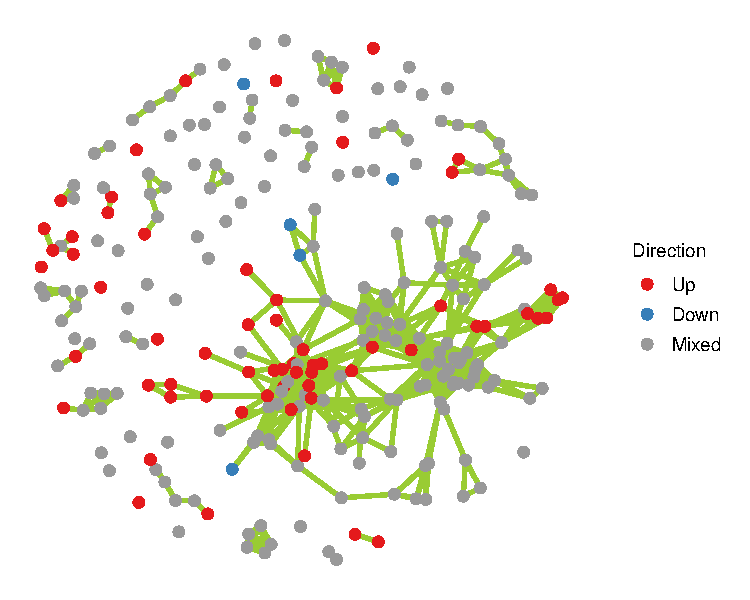
\includegraphics{RICHNET_ms_files/figure-latex/figure1-1} 

}

\caption{Graphical representation of the initial gene set network. Node colors indicate whether the member genes of a set are predominantly up or down regulated or whether there is no preferential direction (mixed).}\label{fig:figure1}
\end{figure}

\section{Network modifications}\label{network-modifications}

In the following, components of the network for which network analysis does not improve interpretability are identified and put to aside. This includes singletons, i.e., genesets not connected to any other geneset, and doublets, also termed binary systems or dumbbells, i.e., pairs of genesets connected with each other but isolated from the rest.

\subsubsection{Identify singletons}\label{identify-singletons}

\begin{Shaded}
\begin{Highlighting}[]
\NormalTok{singletons =}\StringTok{ }\KeywordTok{which}\NormalTok{(igraph}\OperatorTok{::}\KeywordTok{degree}\NormalTok{(net) }\OperatorTok{==}\StringTok{ }\DecValTok{0}\NormalTok{)}
\NormalTok{net1 =}\StringTok{ }\KeywordTok{delete_vertices}\NormalTok{(net, singletons)}
\NormalTok{in.single =}\StringTok{ }\KeywordTok{which}\NormalTok{(dat}\OperatorTok{$}\NormalTok{name }\OperatorTok\StringTok{ }\KeywordTok{V}\NormalTok{(net)}\OperatorTok{$}\NormalTok{name[singletons])}
\NormalTok{tab =}\StringTok{ }\NormalTok{dat[in.single, ]}
\NormalTok{tab}\OperatorTok{$}\NormalTok{FDR =}\StringTok{ }\KeywordTok{signif}\NormalTok{(tab}\OperatorTok{$}\NormalTok{FDR, }\DecValTok{2}\NormalTok{)}
\NormalTok{tab}\OperatorTok{$}\NormalTok{name =}\StringTok{ }\KeywordTok{gsub}\NormalTok{(}\StringTok{"_"}\NormalTok{, }\StringTok{" "}\NormalTok{, tab}\OperatorTok{$}\NormalTok{name)}
\NormalTok{tab =}\StringTok{ }\KeywordTok{kable}\NormalTok{(tab[,}\KeywordTok{c}\NormalTok{(}\StringTok{"name"}\NormalTok{, }\StringTok{"NGenes"}\NormalTok{, }\StringTok{"Direction"}\NormalTok{, }\StringTok{"FDR"}\NormalTok{)], }
            \DataTypeTok{row.names =}\NormalTok{ F, }\DataTypeTok{format =} \StringTok{"latex"}\NormalTok{, }
            \DataTypeTok{caption =} \StringTok{"List of all singletons, i.e., genesets without }
\StringTok{            sufficient overlap with any other geneset."}\NormalTok{)}
\KeywordTok{kable_styling}\NormalTok{(tab, }\DataTypeTok{latex_options =} \StringTok{"scale_down"}\NormalTok{, }\DataTypeTok{font_size =} \DecValTok{8}\NormalTok{)}
\end{Highlighting}
\end{Shaded}

\begin{table}[t]

\caption{\label{tab:singletons}List of all singletons, i.e., genesets without 
            sufficient overlap with any other geneset.}
\centering
\resizebox{\linewidth}{!}{
\fontsize{8}{10}\selectfont
\begin{tabular}{l|r|l|r}
\hline
name & NGenes & Direction & FDR\\
\hline
KEGG GLYCOLYSIS GLUCONEOGENESIS & 58 & Mixed & 0.04900\\
\hline
KEGG GLYCINE SERINE AND THREONINE METABOLISM & 29 & Mixed & 0.00020\\
\hline
KEGG ARGININE AND PROLINE METABOLISM & 52 & Up & 0.04100\\
\hline
KEGG GLUTATHIONE METABOLISM & 43 & Mixed & 0.00210\\
\hline
KEGG O GLYCAN BIOSYNTHESIS & 26 & Mixed & 0.01300\\
\hline
KEGG ARACHIDONIC ACID METABOLISM & 48 & Mixed & 0.04300\\
\hline
KEGG NICOTINATE AND NICOTINAMIDE METABOLISM & 23 & Mixed & 0.00290\\
\hline
KEGG CHEMOKINE SIGNALING PATHWAY & 160 & Mixed & 0.02700\\
\hline
KEGG P53 SIGNALING PATHWAY & 67 & Mixed & 0.01400\\
\hline
KEGG APOPTOSIS & 78 & Mixed & 0.02800\\
\hline
KEGG TGF BETA SIGNALING PATHWAY & 82 & Mixed & 0.00140\\
\hline
KEGG ADHERENS JUNCTION & 72 & Up & 0.02900\\
\hline
KEGG LEUKOCYTE TRANSENDOTHELIAL MIGRATION & 99 & Mixed & 0.00360\\
\hline
KEGG PROGESTERONE MEDIATED OOCYTE MATURATION & 80 & Mixed & 0.04900\\
\hline
KEGG ADIPOCYTOKINE SIGNALING PATHWAY & 62 & Up & 0.00180\\
\hline
KEGG PATHOGENIC ESCHERICHIA COLI INFECTION & 53 & Mixed & 0.04000\\
\hline
BIOCARTA AGR PATHWAY & 33 & Mixed & 0.01300\\
\hline
BIOCARTA ATM PATHWAY & 20 & Mixed & 0.00790\\
\hline
BIOCARTA BCELLSURVIVAL PATHWAY & 15 & Up & 0.03400\\
\hline
BIOCARTA LAIR PATHWAY & 14 & Mixed & 0.00910\\
\hline
BIOCARTA EPONFKB PATHWAY & 11 & Mixed & 0.01300\\
\hline
BIOCARTA GABA PATHWAY & 6 & Mixed & 0.04800\\
\hline
BIOCARTA P53HYPOXIA PATHWAY & 22 & Mixed & 0.02600\\
\hline
BIOCARTA EGFR SMRTE PATHWAY & 11 & Mixed & 0.01600\\
\hline
BIOCARTA PPARA PATHWAY & 52 & Mixed & 0.00091\\
\hline
BIOCARTA RAC1 PATHWAY & 20 & Mixed & 0.00440\\
\hline
BIOCARTA NKCELLS PATHWAY & 14 & Mixed & 0.02800\\
\hline
REACTOME METABOLISM OF VITAMINS AND COFACTORS & 50 & Mixed & 0.03100\\
\hline
REACTOME IL 7 SIGNALING & 10 & Mixed & 0.00062\\
\hline
REACTOME SULFUR AMINO ACID METABOLISM & 24 & Up & 0.00530\\
\hline
REACTOME SPHINGOLIPID DE NOVO BIOSYNTHESIS & 30 & Mixed & 0.00970\\
\hline
REACTOME SIGNALING BY HIPPO & 20 & Mixed & 0.00110\\
\hline
REACTOME GASTRIN CREB SIGNALLING PATHWAY VIA PKC AND MAPK & 171 & Mixed & 0.05000\\
\hline
REACTOME PLATELET ADHESION TO EXPOSED COLLAGEN & 10 & Mixed & 0.00910\\
\hline
REACTOME VEGF LIGAND RECEPTOR INTERACTIONS & 10 & Mixed & 0.05000\\
\hline
REACTOME METABOLISM OF AMINO ACIDS AND DERIVATIVES & 182 & Mixed & 0.03100\\
\hline
REACTOME TRANSMISSION ACROSS CHEMICAL SYNAPSES & 161 & Mixed & 0.01900\\
\hline
REACTOME INTEGRATION OF ENERGY METABOLISM & 104 & Mixed & 0.02900\\
\hline
REACTOME CYTOSOLIC TRNA AMINOACYLATION & 24 & Down & 0.03000\\
\hline
REACTOME OLFACTORY SIGNALING PATHWAY & 65 & Mixed & 0.00220\\
\hline
REACTOME SEMA3A PLEXIN REPULSION SIGNALING BY INHIBITING INTEGRIN ADHESION & 13 & Mixed & 0.04000\\
\hline
REACTOME NA CL DEPENDENT NEUROTRANSMITTER TRANSPORTERS & 12 & Down & 0.03700\\
\hline
REACTOME SYNTHESIS AND INTERCONVERSION OF NUCLEOTIDE DI AND TRIPHOSPHATES & 18 & Up & 0.04700\\
\hline
REACTOME ROLE OF DCC IN REGULATING APOPTOSIS & 10 & Mixed & 0.00420\\
\hline
REACTOME NETRIN1 SIGNALING & 35 & Mixed & 0.00940\\
\hline
REACTOME NEPHRIN INTERACTIONS & 17 & Up & 0.03000\\
\hline
REACTOME RAP1 SIGNALLING & 15 & Mixed & 0.00900\\
\hline
REACTOME ETHANOL OXIDATION & 10 & Up & 0.00012\\
\hline
REACTOME HORMONE SENSITIVE LIPASE HSL MEDIATED TRIACYLGLYCEROL HYDROLYSIS & 11 & Mixed & 0.01000\\
\hline
\end{tabular}}
\end{table}

In total, 49 singletons were identified and excluded from further analyis (Table \ref{tab:singletons}). It is important to note that these genesets, while down-prioritized for the time being, may still be worthwile investigating later.

\begin{figure}

{\centering 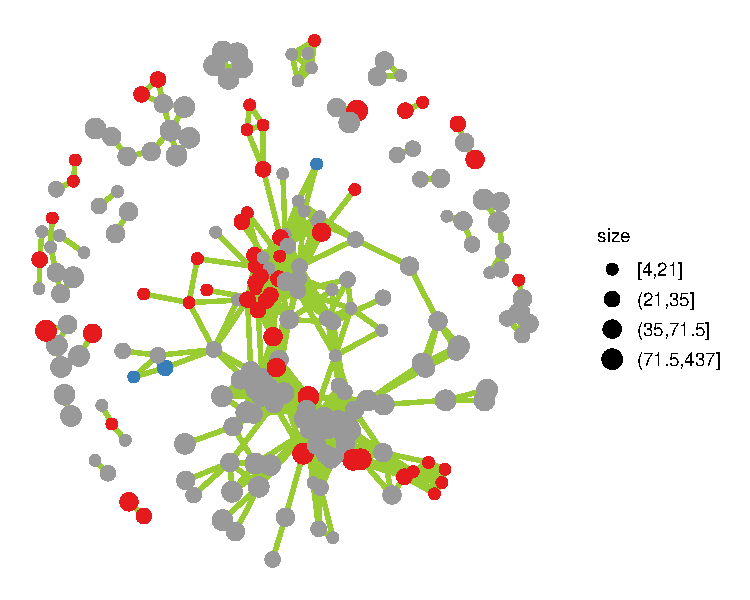
\includegraphics{RICHNET_ms_files/figure-latex/figure2-1} 

}

\caption{Gene set network with singletons removed. The color scheme is the same as above. The node size corresponds to the number of genes in a set.}\label{fig:figure2}
\end{figure}

\begin{Shaded}
\begin{Highlighting}[]
\KeywordTok{ggnet2}\NormalTok{(net1, }\DataTypeTok{size =} \StringTok{"size"}\NormalTok{, }\DataTypeTok{max_size =} \DecValTok{4}\NormalTok{, }\DataTypeTok{color =}\NormalTok{ palette[}\KeywordTok{V}\NormalTok{(net1)}\OperatorTok{$}\NormalTok{Direction], }
       \DataTypeTok{size.cut =} \DecValTok{4}\NormalTok{, }\DataTypeTok{edge.size =} \DecValTok{1}\NormalTok{, }\DataTypeTok{edge.color =} \StringTok{"#99CC33"}\NormalTok{)}
\end{Highlighting}
\end{Shaded}

Figure \ref{fig:figure2} shows the remaining network clusters with the size of the nodes representing the number of genes in the set.

\subsubsection{Identify binary systems (2 sets)}\label{identify-binary-systems-2-sets}

Next we also want to separate clusters with less than 3 gene sets. To do so, we separate disjoint subnets as individual objects, count their members, and delete all vertices belonging to clusters of size smaller than 3.

\begin{Shaded}
\begin{Highlighting}[]
\NormalTok{clu1 =}\StringTok{ }\NormalTok{igraph}\OperatorTok{::}\KeywordTok{components}\NormalTok{(net1)}
\NormalTok{clu.lt3 =}\StringTok{ }\KeywordTok{which}\NormalTok{(}\KeywordTok{sizes}\NormalTok{(clu1) }\OperatorTok{<}\StringTok{ }\DecValTok{3}\NormalTok{)}
\NormalTok{v.clu.lt3 =}\StringTok{ }\KeywordTok{which}\NormalTok{(clu1}\OperatorTok{$}\NormalTok{membership }\OperatorTok\StringTok{ }\NormalTok{clu.lt3)}
\NormalTok{net2 =}\StringTok{ }\KeywordTok{delete_vertices}\NormalTok{(net1, v.clu.lt3)}
\NormalTok{clu2 =}\StringTok{ }\NormalTok{igraph}\OperatorTok{::}\KeywordTok{components}\NormalTok{(net2)}
\NormalTok{in.clu.lt3 =}\StringTok{ }\KeywordTok{which}\NormalTok{(dat}\OperatorTok{$}\NormalTok{name }\OperatorTok\StringTok{ }\KeywordTok{V}\NormalTok{(net1)}\OperatorTok{$}\NormalTok{name[v.clu.lt3])}
\NormalTok{tab =}\StringTok{ }\NormalTok{dat[in.clu.lt3, ]}
\NormalTok{tab}\OperatorTok{$}\NormalTok{FDR =}\StringTok{ }\KeywordTok{signif}\NormalTok{(tab}\OperatorTok{$}\NormalTok{FDR,}\DecValTok{2}\NormalTok{)}
\NormalTok{cludp =}\StringTok{ }\NormalTok{clu1}\OperatorTok{$}\NormalTok{membership[v.clu.lt3]}
\NormalTok{cludp =}\StringTok{ }\KeywordTok{data.frame}\NormalTok{(}\DataTypeTok{name =} \KeywordTok{names}\NormalTok{(cludp), }\DataTypeTok{id =} \KeywordTok{as.numeric}\NormalTok{(cludp))}
\NormalTok{tab =}\StringTok{ }\KeywordTok{merge}\NormalTok{(tab,cludp)}
\NormalTok{tab}\OperatorTok{$}\NormalTok{name =}\StringTok{ }\KeywordTok{gsub}\NormalTok{(}\StringTok{"_"}\NormalTok{, }\StringTok{" "}\NormalTok{, tab}\OperatorTok{$}\NormalTok{name)}
\NormalTok{tab =}\StringTok{ }\KeywordTok{kable}\NormalTok{(tab[}\KeywordTok{order}\NormalTok{(tab}\OperatorTok{$}\NormalTok{id), }\KeywordTok{c}\NormalTok{(}\StringTok{"id"}\NormalTok{, }\StringTok{"name"}\NormalTok{, }\StringTok{"NGenes"}\NormalTok{, }\StringTok{"Direction"}\NormalTok{, }\StringTok{"FDR"}\NormalTok{)], }
            \DataTypeTok{row.names=}\NormalTok{F, }\DataTypeTok{format =} \StringTok{"latex"}\NormalTok{, }
            \DataTypeTok{caption =} \StringTok{"List of binary clusters as indicated by the id column."}\NormalTok{)}
\KeywordTok{kable_styling}\NormalTok{(tab, }\DataTypeTok{latex_options =} \StringTok{"scale_down"}\NormalTok{, }\DataTypeTok{font_size =} \DecValTok{8}\NormalTok{)}
\end{Highlighting}
\end{Shaded}

\newpage

\begin{table}[t]

\caption{\label{tab:binaryclusters}List of binary clusters as indicated by the id column.}
\centering
\resizebox{\linewidth}{!}{
\fontsize{8}{10}\selectfont
\begin{tabular}{r|l|r|l|r}
\hline
id & name & NGenes & Direction & FDR\\
\hline
3 & KEGG ALANINE ASPARTATE AND GLUTAMATE METABOLISM & 28 & Mixed & 4.9e-03\\
\hline
3 & REACTOME AMINO ACID SYNTHESIS AND INTERCONVERSION TRANSAMINATION & 16 & Mixed & 3.6e-04\\
\hline
6 & KEGG INOSITOL PHOSPHATE METABOLISM & 49 & Mixed & 2.0e-04\\
\hline
6 & KEGG PHOSPHATIDYLINOSITOL SIGNALING SYSTEM & 69 & Mixed & 1.5e-04\\
\hline
17 & BIOCARTA ARF PATHWAY & 16 & Mixed & 1.2e-02\\
\hline
17 & BIOCARTA CTCF PATHWAY & 22 & Mixed & 3.8e-04\\
\hline
18 & REACTOME PLATELET ACTIVATION SIGNALING AND AGGREGATION & 178 & Mixed & 2.9e-03\\
\hline
18 & REACTOME RESPONSE TO ELEVATED PLATELET CYTOSOLIC CA2 & 72 & Mixed & 3.9e-02\\
\hline
19 & REACTOME NEUROTRANSMITTER RELEASE CYCLE & 28 & Up & 1.4e-02\\
\hline
19 & REACTOME NOREPINEPHRINE NEUROTRANSMITTER RELEASE CYCLE & 10 & Up & 4.5e-02\\
\hline
20 & REACTOME AMINO ACID AND OLIGOPEPTIDE SLC TRANSPORTERS & 40 & Mixed & 2.0e-02\\
\hline
20 & REACTOME AMINO ACID TRANSPORT ACROSS THE PLASMA MEMBRANE & 29 & Mixed & 8.7e-03\\
\hline
22 & REACTOME MUSCLE CONTRACTION & 42 & Up & 3.4e-05\\
\hline
22 & REACTOME SMOOTH MUSCLE CONTRACTION & 23 & Up & 0.0e+00\\
\hline
23 & REACTOME ACTIVATION OF GENES BY ATF4 & 24 & Mixed & 7.8e-03\\
\hline
23 & REACTOME PERK REGULATED GENE EXPRESSION & 27 & Mixed & 2.0e-02\\
\hline
\end{tabular}}
\end{table}

In Table \ref{tab:binaryclusters}, consecutively listed gene sets with the same \emph{id} belong to the same binary cluster. Often these are gene sets from different libraries describing the same biological process or phenotype. In total, 16 binary clusters were identified, for which network analysis would not be useful.

\begin{Shaded}
\begin{Highlighting}[]
\KeywordTok{set.seed}\NormalTok{(}\DecValTok{16}\NormalTok{)}
\NormalTok{nodecol =}\StringTok{ }\KeywordTok{colorRampPalette}\NormalTok{(}\KeywordTok{brewer.pal}\NormalTok{(}\DecValTok{9}\NormalTok{, }\StringTok{"Set1"}\NormalTok{)[}\KeywordTok{sample}\NormalTok{(}\DecValTok{9}\NormalTok{)])(}\KeywordTok{max}\NormalTok{(clu2}\OperatorTok{$}\NormalTok{membership))}
\KeywordTok{ggnet2}\NormalTok{(net2, }\DataTypeTok{size =} \StringTok{"size"}\NormalTok{, }\DataTypeTok{max_size =} \DecValTok{4}\NormalTok{, }\DataTypeTok{color =}\NormalTok{ nodecol[clu2}\OperatorTok{$}\NormalTok{membership], }
       \DataTypeTok{size.cut =} \DecValTok{4}\NormalTok{, }\DataTypeTok{edge.size =} \DecValTok{1}\NormalTok{, }\DataTypeTok{edge.color =} \StringTok{"grey"}\NormalTok{) }
\end{Highlighting}
\end{Shaded}

\begin{figure}

{\centering 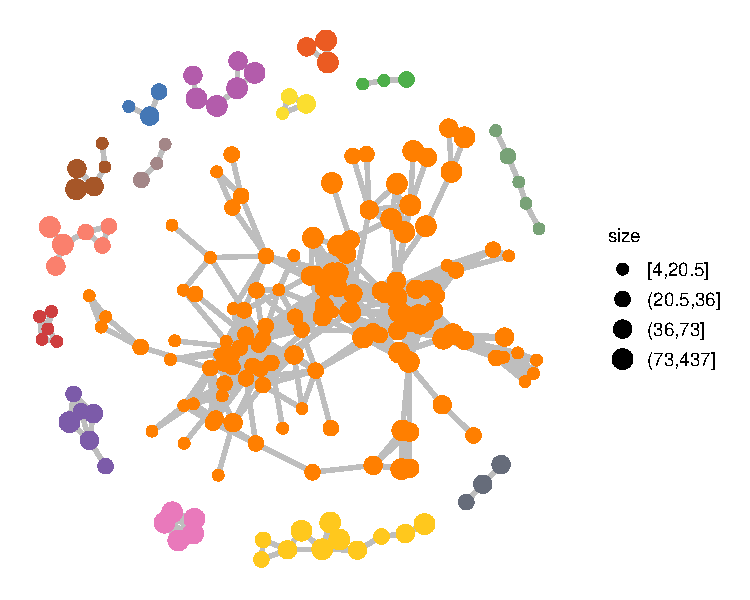
\includegraphics{RICHNET_ms_files/figure-latex/figure3-1} 

}

\caption{Gene set network with singletons and binary clusters removed. Colored according to disjoint subnetworks.}\label{fig:figure3}
\end{figure}

Without singletons and binary clusters, we are left with larger disjoint subnets (Figure \ref{fig:figure3}).

\subsubsection{Detect communities (sub-networks)}\label{detect-communities-sub-networks}

The larger disjoint clusters may consist of so-called \emph{communities}, i.e., sub-networks of highly inter-connected nodes that stick together by only one or a few edges. We are using the popular \emph{edge betweenness} property to identify these community-connecting edges and remove them in order to split large clusters into smaller ones.

\begin{Shaded}
\begin{Highlighting}[]
\NormalTok{net2 =}\StringTok{ }\KeywordTok{delete_edge_attr}\NormalTok{(net2, }\StringTok{"weight"}\NormalTok{)}
\NormalTok{clu3 =}\StringTok{ }\KeywordTok{cluster_edge_betweenness}\NormalTok{(net2)}
\CommentTok{# delete edges between communities}
\NormalTok{net3 =}\StringTok{ }\KeywordTok{delete_edges}\NormalTok{(net2, }\KeywordTok{which}\NormalTok{(}\KeywordTok{as.vector}\NormalTok{(}\KeywordTok{crossing}\NormalTok{(clu3, net2))) )}
\CommentTok{# remove clusters of size <3}
\NormalTok{small_cluster_ids =}\StringTok{ }\KeywordTok{which}\NormalTok{(}\KeywordTok{sizes}\NormalTok{(clu3) }\OperatorTok{<}\StringTok{ }\DecValTok{3}\NormalTok{)}
\NormalTok{small_cl_v =}\StringTok{ }\KeywordTok{which}\NormalTok{(clu3}\OperatorTok{$}\NormalTok{membership }\OperatorTok\StringTok{ }\NormalTok{small_cluster_ids)}
\NormalTok{net3 =}\StringTok{ }\KeywordTok{delete_vertices}\NormalTok{(net3, small_cl_v)}

\NormalTok{clu3 =}\StringTok{ }\NormalTok{igraph}\OperatorTok{::}\KeywordTok{components}\NormalTok{(net3)}
\NormalTok{nodecol =}\StringTok{ }\KeywordTok{c}\NormalTok{(}\KeywordTok{brewer.pal}\NormalTok{(}\DecValTok{9}\NormalTok{, }\StringTok{"Paired"}\NormalTok{), }\KeywordTok{brewer.pal}\NormalTok{(}\DecValTok{9}\NormalTok{, }\StringTok{"Set3"}\NormalTok{) )}
\NormalTok{nodecol =}\StringTok{ }\KeywordTok{colorRampPalette}\NormalTok{(nodecol)(}\KeywordTok{max}\NormalTok{(clu3}\OperatorTok{$}\NormalTok{membership))}
\end{Highlighting}
\end{Shaded}

\begin{Shaded}
\begin{Highlighting}[]
\KeywordTok{ggnet2}\NormalTok{(net3, }\DataTypeTok{size =} \DecValTok{0}\NormalTok{, }\DataTypeTok{color =}\NormalTok{ nodecol[clu3}\OperatorTok{$}\NormalTok{membership], }
       \DataTypeTok{edge.size =} \FloatTok{1.0}\NormalTok{, }\DataTypeTok{edge.color =} \StringTok{"grey"}\NormalTok{) }\OperatorTok{+}\StringTok{ }
\StringTok{  }\KeywordTok{geom_point}\NormalTok{(}\DataTypeTok{size =} \DecValTok{2}\NormalTok{, }\DataTypeTok{color =} \StringTok{"black"}\NormalTok{) }\OperatorTok{+}\StringTok{ }
\StringTok{  }\KeywordTok{geom_point}\NormalTok{(}\KeywordTok{aes}\NormalTok{(}\DataTypeTok{color =}\NormalTok{ color), }\DataTypeTok{size =} \DecValTok{1}\NormalTok{)}
\end{Highlighting}
\end{Shaded}

\begin{figure}

{\centering 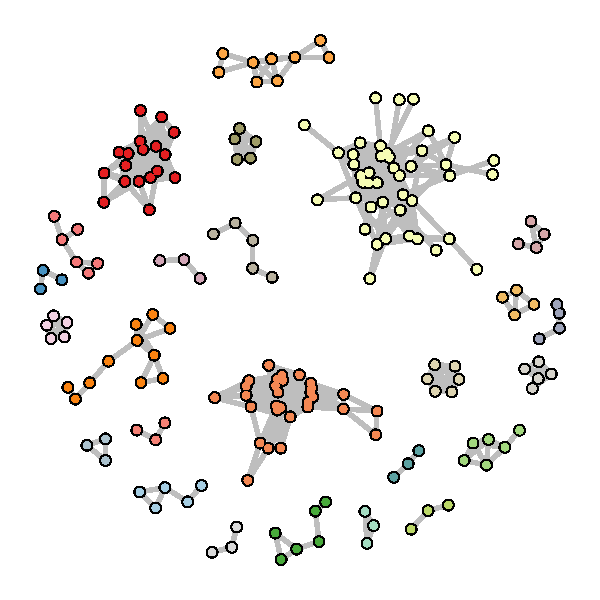
\includegraphics{RICHNET_ms_files/figure-latex/figure4-1} 

}

\caption{Disjoint clusters after community detection and splitting.}\label{fig:figure4}
\end{figure}

The result of this network-based clustering is shown in Fig. \ref{fig:figure4}

\newpage

\section{Automatic annotation of gene set clusters}\label{automatic-annotation-of-gene-set-clusters}

In analogy to the popular interactive network visualization tool \emph{cytoscape} \citep{Kucera2016}, we attempt to generate automatic labels for gene set clusters. Gene set names are split into individual words and counted within each cluster. The four most frequent terms occuring at least twice are used as labels. The function \texttt{clust\_head()} is defined for this purpose and contains an exclusion list of words not used.

\begin{Shaded}
\begin{Highlighting}[]
\NormalTok{t.rW =}\StringTok{ }\KeywordTok{c}\NormalTok{(}\StringTok{"cell"}\NormalTok{, }\StringTok{"process"}\NormalTok{, }\StringTok{"regulation"}\NormalTok{, }\StringTok{"negative"}\NormalTok{, }\StringTok{"positive"}\NormalTok{, }\StringTok{"signaling"}\NormalTok{, }
         \StringTok{"response"}\NormalTok{, }\StringTok{"stimulus"}\NormalTok{, }\StringTok{"signal"}\NormalTok{, }\StringTok{"activity"}\NormalTok{, }\StringTok{"protein"}\NormalTok{, }\StringTok{"involved"}\NormalTok{, }
         \StringTok{"component"}\NormalTok{, }\StringTok{"level"}\NormalTok{, }\StringTok{"effector"}\NormalTok{, }\StringTok{"event"}\NormalTok{, }\StringTok{"projection"}\NormalTok{, }\StringTok{"organismal"}\NormalTok{, }
         \StringTok{"cellular"}\NormalTok{, }\StringTok{"modification"}\NormalTok{, }\StringTok{"pathway"}\NormalTok{, }\StringTok{"mediated"}\NormalTok{, }\StringTok{"dependent"}\NormalTok{, }
         \StringTok{"organization"}\NormalTok{, }\StringTok{"group"}\NormalTok{, }\StringTok{"target"}\NormalTok{, }\StringTok{"biocarta"}\NormalTok{, }\StringTok{"kegg"}\NormalTok{, }\StringTok{"reactome"}\NormalTok{)}
\NormalTok{clust_head =}\StringTok{ }\ControlFlowTok{function}\NormalTok{(x)\{}
\NormalTok{  txt =}\StringTok{ }\KeywordTok{unlist}\NormalTok{(}\KeywordTok{strsplit}\NormalTok{(x, }\StringTok{"_"}\NormalTok{))}
\NormalTok{  txt =}\StringTok{ }\KeywordTok{Corpus}\NormalTok{(}\KeywordTok{VectorSource}\NormalTok{(txt))}
\NormalTok{  txt =}\StringTok{ }\KeywordTok{tm_map}\NormalTok{(txt, PlainTextDocument)}
\NormalTok{  txt =}\StringTok{ }\KeywordTok{tm_map}\NormalTok{(txt, removePunctuation)}
\NormalTok{  txt =}\StringTok{ }\KeywordTok{tm_map}\NormalTok{(txt, removeNumbers)}
\NormalTok{  txt =}\StringTok{ }\KeywordTok{tm_map}\NormalTok{(txt, }\KeywordTok{content_transformer}\NormalTok{(tolower))}
\NormalTok{  txt =}\StringTok{ }\KeywordTok{tm_map}\NormalTok{(txt, removeWords, }\KeywordTok{c}\NormalTok{(t.rW, }\KeywordTok{stopwords}\NormalTok{(}\StringTok{"english"}\NormalTok{)))}
\NormalTok{  tdm =}\StringTok{ }\KeywordTok{TermDocumentMatrix}\NormalTok{(txt)}
\NormalTok{  m =}\StringTok{ }\KeywordTok{as.matrix}\NormalTok{(tdm)}
\NormalTok{  word_freqs =}\StringTok{ }\KeywordTok{sort}\NormalTok{(}\KeywordTok{rowSums}\NormalTok{(m), }\DataTypeTok{decreasing=}\OtherTok{TRUE}\NormalTok{) }
\NormalTok{  word_freqs =}\StringTok{ }\NormalTok{word_freqs[word_freqs}\OperatorTok{>}\DecValTok{1}\NormalTok{]}
\NormalTok{  word_freqs =}\StringTok{ }\KeywordTok{paste}\NormalTok{(}\KeywordTok{names}\NormalTok{(word_freqs)[}\DecValTok{1}\OperatorTok{:}\DecValTok{4}\NormalTok{], }\DataTypeTok{collapse=}\StringTok{" "}\NormalTok{)}
  \KeywordTok{gsub}\NormalTok{(}\StringTok{"[[:space:]]?NA[[:space:]]?"}\NormalTok{, }\StringTok{""}\NormalTok{, word_freqs)}
\NormalTok{\}}
\end{Highlighting}
\end{Shaded}

\subsubsection{Lattice of annotated networks}\label{lattice-of-annotated-networks}

There are many possiblities to visualize geneset clusters and often a compromize between information content and crowding has to be found. Here, we are producing a lattice of network plots, one for each sub-net, with the automatic annotation as title. We begin by generating the cluster titles using the \texttt{clust\_head()} function followed by cleaning up and ordering by cluster size.

\begin{Shaded}
\begin{Highlighting}[]
\NormalTok{clust =}\StringTok{ }\KeywordTok{data.frame}\NormalTok{(}\DataTypeTok{cl =}\NormalTok{ clu3}\OperatorTok{$}\NormalTok{membership)}
\KeywordTok{rownames}\NormalTok{(clust) =}\StringTok{ }\KeywordTok{names}\NormalTok{(}\KeywordTok{V}\NormalTok{(net3))}
\CommentTok{# generate cluster titles }
\NormalTok{cl3.lab.txt =}\StringTok{ }\KeywordTok{as.character}\NormalTok{(}\KeywordTok{tapply}\NormalTok{(}\KeywordTok{rownames}\NormalTok{(clust), clust}\OperatorTok{$}\NormalTok{cl, clust_head))}
\CommentTok{# remove NAs }
\NormalTok{cl3.lab.txt =}\StringTok{ }\KeywordTok{gsub}\NormalTok{(}\StringTok{"[[:space:]]?NA[[:space:]]?"}\NormalTok{, }\StringTok{""}\NormalTok{, cl3.lab.txt)}
\NormalTok{clu3 =}\StringTok{ }\NormalTok{igraph}\OperatorTok{::}\KeywordTok{components}\NormalTok{(net3)}
\NormalTok{clu.order =}\StringTok{ }\KeywordTok{order}\NormalTok{(clu3}\OperatorTok{$}\NormalTok{csize, }\DataTypeTok{decreasing =}\NormalTok{ T)}
\NormalTok{clu3}\OperatorTok{$}\NormalTok{mem =}\StringTok{ }\KeywordTok{match}\NormalTok{(clu3}\OperatorTok{$}\NormalTok{membership, clu.order)}
\end{Highlighting}
\end{Shaded}

Then we generate a list of ggplot objects, one for each cluster or sub-net. For smaller sub-nets, the nodes are labelled with the first 4 words of their names; the first word was removed before as it is usually the name of the geneset library. For larger sub-nets, this is not feasible without overprinting. Titles are missing if none of the words from the geneset names occured more than once.

\begin{Shaded}
\begin{Highlighting}[]
\CommentTok{# generate a list of ggplots}
\NormalTok{g =}\StringTok{ }\KeywordTok{list}\NormalTok{(}\KeywordTok{max}\NormalTok{(clu3}\OperatorTok{$}\NormalTok{membership))}
\KeywordTok{set.seed}\NormalTok{(}\DecValTok{7042016}\NormalTok{)}
\ControlFlowTok{for}\NormalTok{ (ii }\ControlFlowTok{in} \DecValTok{1}\OperatorTok{:}\KeywordTok{max}\NormalTok{(clu3}\OperatorTok{$}\NormalTok{membership)) \{}
\NormalTok{  subgf =}\StringTok{ }\KeywordTok{induced_subgraph}\NormalTok{(net3, }\KeywordTok{which}\NormalTok{(clu3}\OperatorTok{$}\NormalTok{mem }\OperatorTok{==}\StringTok{ }\NormalTok{ii))}
  \CommentTok{# generate titles with one optional line break}
\NormalTok{  title =}\StringTok{ }\KeywordTok{substr}\NormalTok{(}\KeywordTok{toupper}\NormalTok{(cl3.lab.txt[clu.order][ii]), }\DecValTok{1}\NormalTok{, }\DecValTok{60}\NormalTok{)}
  \ControlFlowTok{if}\NormalTok{ (}\KeywordTok{nchar}\NormalTok{(title) }\OperatorTok{>}\StringTok{ }\DecValTok{25}\NormalTok{) \{}
\NormalTok{    title =}\StringTok{ }\KeywordTok{sub}\NormalTok{(}\StringTok{"(^.\{10,30\})[[:space:]]"}\NormalTok{,}\StringTok{"}\CharTok{\textbackslash{}\textbackslash{}}\StringTok{1}\CharTok{\textbackslash{}\textbackslash{}\textbackslash{}n}\StringTok{"}\NormalTok{, title)}
\NormalTok{  \}}
  \CommentTok{# generate node labels using word 2-5 of the geneset name}
\NormalTok{  v.label =}\StringTok{ }\KeywordTok{names}\NormalTok{(}\KeywordTok{V}\NormalTok{(subgf))}
\NormalTok{  v.label =}\StringTok{ }\KeywordTok{lapply}\NormalTok{(v.label, }\ControlFlowTok{function}\NormalTok{(x) }\KeywordTok{strsplit}\NormalTok{(x, }\StringTok{"_"}\NormalTok{)[[}\DecValTok{1}\NormalTok{]])}
\NormalTok{  v.label =}\StringTok{ }\KeywordTok{sapply}\NormalTok{(v.label, }\ControlFlowTok{function}\NormalTok{(x) }\KeywordTok{paste}\NormalTok{(x[}\DecValTok{2}\OperatorTok{:}\KeywordTok{min}\NormalTok{(}\DecValTok{5}\NormalTok{, }\KeywordTok{length}\NormalTok{(x))], }
                                              \DataTypeTok{collapse =} \StringTok{"_"}\NormalTok{))}
  \CommentTok{# clean up geneset names}
\NormalTok{  v.label =}\StringTok{  }\KeywordTok{gsub}\NormalTok{(}\StringTok{"_PATHWAY"}\NormalTok{,}\StringTok{""}\NormalTok{, v.label)}
\NormalTok{  v.label =}\StringTok{  }\KeywordTok{gsub}\NormalTok{(}\StringTok{"_SIGNALING"}\NormalTok{, }\StringTok{""}\NormalTok{, v.label)}
  \CommentTok{# introduce line breaks}
\NormalTok{  v.label =}\StringTok{  }\KeywordTok{gsub}\NormalTok{(}\StringTok{"_"}\NormalTok{,}\StringTok{"}\CharTok{\textbackslash{}n}\StringTok{"}\NormalTok{, v.label)}
  \CommentTok{# remove node labels for large clusters}
  \ControlFlowTok{if}\NormalTok{ (}\KeywordTok{length}\NormalTok{(v.label) }\OperatorTok{>}\StringTok{ }\DecValTok{5}\NormalTok{) v.label =}\StringTok{ }\KeywordTok{rep}\NormalTok{(}\OtherTok{NA}\NormalTok{, }\KeywordTok{length}\NormalTok{(v.label))}
\NormalTok{  g[[ii]] =}\StringTok{ }\KeywordTok{ggnet2}\NormalTok{(subgf, }\DataTypeTok{edge.size =} \DecValTok{1}\NormalTok{, }\DataTypeTok{edge.color =} \StringTok{"#99CC33"}\NormalTok{,}
                   \DataTypeTok{label =}\NormalTok{ F, }\DataTypeTok{size=}\KeywordTok{V}\NormalTok{(subgf)}\OperatorTok{$}\NormalTok{size, }\DataTypeTok{max_size =} \DecValTok{3}\NormalTok{,}
                   \DataTypeTok{size.cut =} \DecValTok{4}\NormalTok{, }\DataTypeTok{color =}\NormalTok{ palette[}\KeywordTok{V}\NormalTok{(subgf)}\OperatorTok{$}\NormalTok{Direction]) }\OperatorTok{+}
\StringTok{    }\KeywordTok{theme}\NormalTok{(}\DataTypeTok{legend.position=}\StringTok{"none"}\NormalTok{, }\DataTypeTok{plot.title =} \KeywordTok{element_text}\NormalTok{(}\DataTypeTok{size=}\DecValTok{6}\NormalTok{), }
          \DataTypeTok{panel.grid =} \KeywordTok{element_blank}\NormalTok{()) }\OperatorTok{+}\StringTok{ }
\StringTok{    }\KeywordTok{geom_label_repel}\NormalTok{(}\DataTypeTok{label =}\NormalTok{ v.label, }\DataTypeTok{size=}\FloatTok{1.2}\NormalTok{,}
                     \DataTypeTok{box.padding =} \FloatTok{0.1}\NormalTok{, }\DataTypeTok{label.padding =} \FloatTok{0.1}\NormalTok{) }\OperatorTok{+}\StringTok{  }
\StringTok{    }\KeywordTok{ggtitle}\NormalTok{(title) \}}
\end{Highlighting}
\end{Shaded}

\begin{Shaded}
\begin{Highlighting}[]
\NormalTok{nr.cols =}\StringTok{ }\KeywordTok{min}\NormalTok{(}\DecValTok{4}\NormalTok{,}\KeywordTok{max}\NormalTok{(clu3}\OperatorTok{$}\NormalTok{membership))}
\NormalTok{nr.rows =}\StringTok{ }\KeywordTok{ceiling}\NormalTok{(}\KeywordTok{max}\NormalTok{(clu3}\OperatorTok{$}\NormalTok{membership) }\OperatorTok{/}\StringTok{ }\NormalTok{nr.cols)}
\NormalTok{width =}\StringTok{ }\KeywordTok{sapply}\NormalTok{(g, }\ControlFlowTok{function}\NormalTok{(x) }\KeywordTok{nrow}\NormalTok{(x}\OperatorTok{$}\NormalTok{data))}
\NormalTok{grid.arrange =}\StringTok{ }\KeywordTok{getFromNamespace}\NormalTok{(}\StringTok{"grid.arrange"}\NormalTok{, }\KeywordTok{asNamespace}\NormalTok{(}\StringTok{"gridExtra"}\NormalTok{))}
\KeywordTok{grid.arrange}\NormalTok{(}\DataTypeTok{grobs =}\NormalTok{ g[}\KeywordTok{seq}\NormalTok{(}\DecValTok{16}\NormalTok{)], }\DataTypeTok{ncol =}\NormalTok{ nr.cols)}
\end{Highlighting}
\end{Shaded}

\newpage 

\begin{figure}

{\centering 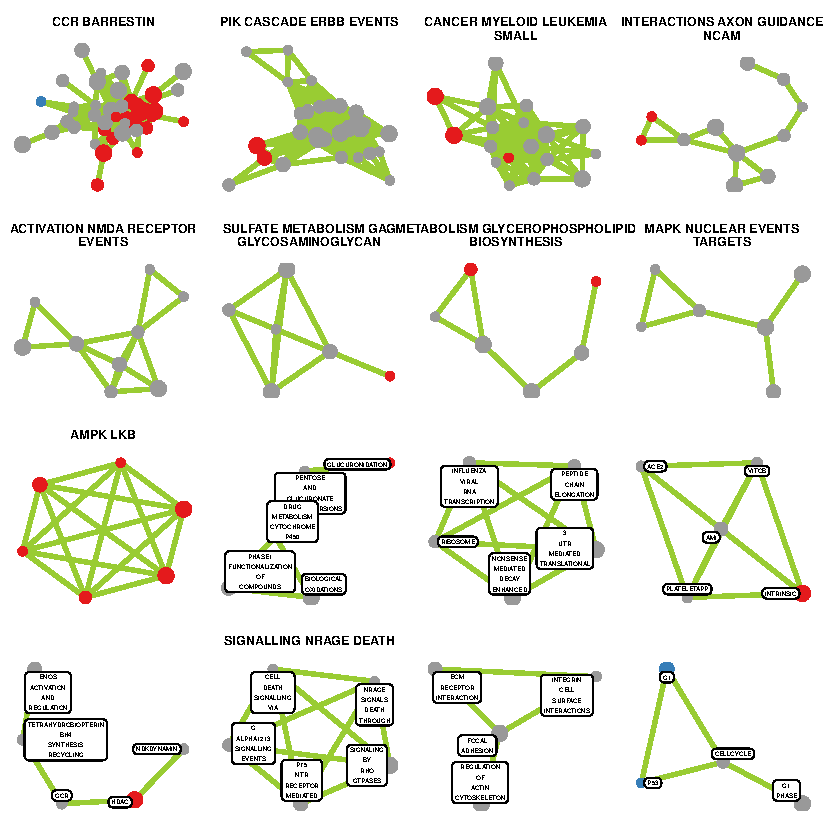
\includegraphics{RICHNET_ms_files/figure-latex/figure5-1} 

}

\caption{Geneset cluster with machine-generated titles. Only the first 16 connected subnets are shown. Geneset labels are omitted for clusters with more than 5 members.}\label{fig:figure5}
\end{figure}\newpage 

\newpage 

\section{Discussion}\label{discussion}

We have presented an automated workflow based on a small number of R packages for prioritization and visualization of gene set analysis results using networks, which we call RICHNET. We demonstrated how community detection facilitates categorization of differentially regulated gene sets into singletons and clusters of different size ranges. Automated label generation allowed to associate these clusters with biological themes or processes of which the member gene sets are part of.

The RICHNET workflow could be altered or extended quite naturally in a number of ways but the version presented here is the one we typically apply in our research service projects. One advantage over other approaches is that it does not depend on a particular genset library. Specific hierarchically constructed genesets, such as GO terms, would offer a straightforward way to arrive at a more global process description using higher levels in their tree structure. A second advantage is that it does not depend on the existence of a good quality gene or protein interaction network for the particular organism or disease state which is often not feasible. Only very few genesets are network-based (e.g.~KEGG pathways) and would thus offer a straight-forward way to use an \emph{i priori} network topology. Thirdly, similar as in \citep{Thorsson2018}, a geneset similarity network could be constructed in the form of a co-enrichment network from GSVA enrichment scores \citep{Hanzelmann2013} using weighted coxpression network analysis (WGCNA) \citep{Langfelder2008}. However, this approach relies on a relatively large sample size whereas the sample size requirement of RICHNET is not more than the GSA it relies on.

As an alternative to the networks of genesets described here, networks of genes could be created in a reciprocal way. The underlying similarity metric between genes could be defined as the proportion of common genesets among all genesets they are part of. This approach would be equivalent to a STRING-DB network with ``databases'' as the only interaction allowed \citep{Szklarczyk2017}.

One possible future extension of the RICHNET workflow could be the introduction of a consensus similarity metric from multiple initial networks and different community detection or cluster algorithms to improve stability against noise. A second avenue forward could be the introduction of interactive graphics in 2D or 3D \citep{Ognyanova2015} to allow moving, pulling, rotation or zoom and display of node specific or edge specific information.

Some may argue in favor of encapsulating the RICHNET workflow in an R or Bioconductor package. However, it is our strong believe that for the sake of transparency and given the straightforward nature of the code it serves better to publish it openly. This way we encourage the users to addapt it to their specific requirements, to improve and expand on it.

\section{Data availability}\label{data-availability}

The data used in this workflow is included in the \emph{airway} R-package\citep{Himes2014}.

\section{Software availability}\label{software-availability}

The R markdown file for this workflow can be \href{https://gitlab.ethz.ch/nexuscbu/richnet/tree/master/RICHNET_ms/RICHNET_ms.Rmd}{downloaded}, used and distributed according to the \href{https://creativecommons.org/licenses/by/4.0/}{Creative Commons CC BY license}.

\newpage 

\begin{Shaded}
\begin{Highlighting}[]
\KeywordTok{sessionInfo}\NormalTok{()}
\end{Highlighting}
\end{Shaded}

R version 3.5.1 (2018-07-02)
Platform: x86\_64-w64-mingw32/x64 (64-bit)
Running under: Windows 10 x64 (build 17134)

Matrix products: default

locale:
{[}1{]} LC\_COLLATE=English\_United Kingdom.1252
{[}2{]} LC\_CTYPE=English\_United Kingdom.1252\\
{[}3{]} LC\_MONETARY=English\_United Kingdom.1252
{[}4{]} LC\_NUMERIC=C\\
{[}5{]} LC\_TIME=English\_United Kingdom.1252

attached base packages:
{[}1{]} parallel stats4 stats graphics grDevices utils datasets
{[}8{]} methods base

other attached packages:
{[}1{]} airway\_1.2.0 SnowballC\_0.5.1\\
{[}3{]} tm\_0.7-6 NLP\_0.2-0\\
{[}5{]} wordcloud\_2.6 org.Hs.eg.db\_3.7.0\\
{[}7{]} AnnotationDbi\_1.44.0 limma\_3.38.3\\
{[}9{]} DESeq2\_1.22.1 SummarizedExperiment\_1.12.0
{[}11{]} DelayedArray\_0.8.0 BiocParallel\_1.16.4\\
{[}13{]} matrixStats\_0.54.0 Biobase\_2.42.0\\
{[}15{]} GenomicRanges\_1.34.0 GenomeInfoDb\_1.18.1\\
{[}17{]} IRanges\_2.16.0 S4Vectors\_0.20.1\\
{[}19{]} BiocGenerics\_0.28.0 GGally\_1.4.0\\
{[}21{]} igraph\_1.2.2 kableExtra\_0.9.0\\
{[}23{]} knitr\_1.21 reshape2\_1.4.3\\
{[}25{]} ggrepel\_0.8.0 cowplot\_0.9.3\\
{[}27{]} gplots\_3.0.1 ggplot2\_3.1.0\\
{[}29{]} RColorBrewer\_1.1-2

loaded via a namespace (and not attached):
{[}1{]} colorspace\_1.3-2 rprojroot\_1.3-2\\
{[}3{]} htmlTable\_1.13 XVector\_0.22.0\\
{[}5{]} base64enc\_0.1-3 fs\_1.2.6\\
{[}7{]} rstudioapi\_0.8 remotes\_2.0.2\\
{[}9{]} bit64\_0.9-7 xml2\_1.2.0\\
{[}11{]} codetools\_0.2-16 splines\_3.5.1\\
{[}13{]} geneplotter\_1.60.0 pkgload\_1.0.2\\
{[}15{]} Formula\_1.2-3 annotate\_1.60.0\\
{[}17{]} cluster\_2.0.7-1 intergraph\_2.0-2\\
{[}19{]} readr\_1.3.1 compiler\_3.5.1\\
{[}21{]} httr\_1.4.0 backports\_1.1.3\\
{[}23{]} assertthat\_0.2.0 Matrix\_1.2-15\\
{[}25{]} lazyeval\_0.2.1 cli\_1.0.1\\
{[}27{]} acepack\_1.4.1 htmltools\_0.3.6\\
{[}29{]} prettyunits\_1.0.2 tools\_3.5.1\\
{[}31{]} bindrcpp\_0.2.2 coda\_0.19-2\\
{[}33{]} gtable\_0.2.0 glue\_1.3.0\\
{[}35{]} GenomeInfoDbData\_1.2.0 dplyr\_0.7.8\\
{[}37{]} BiocWorkflowTools\_1.8.0 Rcpp\_1.0.0\\
{[}39{]} slam\_0.1-44 statnet.common\_4.1.4\\
{[}41{]} gdata\_2.18.0 xfun\_0.4\\
{[}43{]} stringr\_1.3.1 network\_1.13.0.1\\
{[}45{]} ps\_1.3.0 testthat\_2.0.1\\
{[}47{]} rvest\_0.3.2 gtools\_3.8.1\\
{[}49{]} devtools\_2.0.1 XML\_3.98-1.16\\
{[}51{]} zlibbioc\_1.28.0 scales\_1.0.0\\
{[}53{]} hms\_0.4.2 yaml\_2.2.0\\
{[}55{]} memoise\_1.1.0 gridExtra\_2.3\\
{[}57{]} rpart\_4.1-13 RSQLite\_2.1.1\\
{[}59{]} reshape\_0.8.8 latticeExtra\_0.6-28\\
{[}61{]} stringi\_1.2.4 genefilter\_1.64.0\\
{[}63{]} desc\_1.2.0 checkmate\_1.8.5\\
{[}65{]} caTools\_1.17.1.1 pkgbuild\_1.0.2\\
{[}67{]} rlang\_0.3.0.1 pkgconfig\_2.0.2\\
{[}69{]} bitops\_1.0-6 evaluate\_0.12\\
{[}71{]} lattice\_0.20-38 purrr\_0.2.5\\
{[}73{]} bindr\_0.1.1 htmlwidgets\_1.3\\
{[}75{]} bit\_1.1-14 processx\_3.2.1\\
{[}77{]} tidyselect\_0.2.5 plyr\_1.8.4\\
{[}79{]} magrittr\_1.5 bookdown\_0.9\\
{[}81{]} R6\_2.3.0 Hmisc\_4.1-1\\
{[}83{]} sna\_2.4 DBI\_1.0.0\\
{[}85{]} pillar\_1.3.1 foreign\_0.8-71\\
{[}87{]} withr\_2.1.2 survival\_2.43-3\\
{[}89{]} RCurl\_1.95-4.11 nnet\_7.3-12\\
{[}91{]} tibble\_1.4.2 crayon\_1.3.4\\
{[}93{]} KernSmooth\_2.23-15 rmarkdown\_1.11\\
{[}95{]} usethis\_1.4.0 locfit\_1.5-9.1\\
{[}97{]} grid\_3.5.1 data.table\_1.11.8\\
{[}99{]} blob\_1.1.1 callr\_3.1.1\\
{[}101{]} git2r\_0.23.0 digest\_0.6.18\\
{[}103{]} xtable\_1.8-3 munsell\_0.5.0\\
{[}105{]} viridisLite\_0.3.0 sessioninfo\_1.1.1

\section{Author contributions}\label{author-contributions}

MP conceptualized the content, developed the method, performed the analysis and wrote the manuscript.

\section{Competing interests}\label{competing-interests}

No competing interests were disclosed.

\section{Grant information}\label{grant-information}

The author declared that no grants were involved in supporting this work.

\section{Acknowledgments}\label{acknowledgments}

The author would like to thank all members of NEXUS and in particular Daniel Stekhoven for fruitful discussions as well as Beate Sick and Phil Cheng for critically reading the manuscript.

{\small\bibliography{richnet.bib}}

\end{document}
